% Chapter 1: Introduction & Motivation
% Converted from docs/thesis_research_outline.md (Part 1)

\chapter{Introduction \& Motivation}
\label{ch:introduction}

\section{Research Questions}
\label{sec:research-questions}

\textbf{What we empirically observe and measure (high-level):}
\begin{itemize}
    \item \textbf{Cross-model grounding}: Gemini vs.\ ChatGPT
    \item \textbf{Cross-deployment grounding}: ChatGPT \textbf{Personal vs Enterprise}
    \item \textbf{Rank effects}: how grounding/citation choices relate to \textbf{SERP position distributions} (position bias)
    \item \textbf{Selection bias in sources}: differences between the \textbf{available menu} (Top-N SERP) vs the \textbf{selected order} (cited set), measured via \textbf{Content DNA enrichment} of cited and non-cited URLs
    \item \textbf{Visibility gaps}: ``invisible/shadow'' citations (cited URLs missing from the defined Top-N baseline), analyzed separately from within-SERP drift
\end{itemize}

\subsection{Core Research Question}
\label{sec:core-rq}

\textbf{RQ1:} \textit{How does grounding behavior manifest in LLM-generated product recommendations, and how does it vary across conditions we can observe (deployment context and/or model)?}

\subsubsection{Operational Definition (What ``Grounding Behavior'' Means in This Thesis)}
\label{sec:grounding-definition}

Grounding behavior is the measurable pipeline from \textbf{retrieval $\rightarrow$ selection $\rightarrow$ citation $\rightarrow$ final text}, using observable artifacts:
\begin{itemize}
    \item \textbf{Retrieved candidate set} (where available): sources the system pulled/considered
    \item \textbf{Selected set}: sources that ``survive'' selection (cited/attached)
    \item \textbf{Claim linkage}: which textual claims map to which sources (claim-to-link mapping)
    \item \textbf{SERP support}: whether selected sources are actually present in external SERPs (Bing/Google)
    \item \textbf{Source-to-output fidelity}: whether products mentioned in retrieved listicles are carried into the final recommendations
\end{itemize}

\subsection{Sub-questions (Decompositions of RQ1, Not Separate Topics)}
\label{sec:sub-questions}

\begin{itemize}
    \item \textbf{RQ1a (selection + visibility)}: How do \textbf{cited vs additional vs unreferenced/invisible} sources differ in domain/type, and how does this differ by \textbf{enterprise vs personal} runs on ChatGPT results?
    \item \textbf{RQ1b (external support)}: How often do selected citations appear in \textbf{Top-N SERPs} (Bing/Google overlap; Gemini ``survival'' in Top-20)?
    \item \textbf{RQ1c (selection bias \& DNA)}: Does the model exhibit a statistically significant preference for specific \textbf{Content DNA features} (e.g., tables, numbered lists, freshness) when selecting from the retrieved ``Menu,'' and how does this preference vary between \textbf{GPT Personal, GPT Enterprise and Gemini}?
    \item \textbf{RQ1d (listicle uptake / fidelity)}: When listicles are retrieved, which listicle-mentioned products are \textbf{selected vs ignored} in the final response (uptake rate, rank bias, host-bias), and how does this differ by run type?
\end{itemize}

\subsection{Role of External Systems (Clarify Scope)}
\label{sec:external-systems}

\begin{itemize}
    \item \textbf{Bing}: baseline ``human web'' retrieval/ranking surface used as a \textbf{measurement instrument} for rank/visibility and ``visibility gaps'' (\textbf{Top-200}).
    \item \textbf{Google (SerpApi)}: control baseline for Gemini fan-out queries and sensitivity checks (\textbf{Organic-only} vs including non-organic result types like \textbf{Video/PAA/Discussions}).
    \item \textbf{Gemini}: optional cross-model baseline for grounding mechanics (has explicit \texttt{groundingMetadata} and claim-support mapping); not an enterprise/personal split unless we create our own conditions.
\end{itemize}

\section{Market Context \& Motivation (Ahrefs Benchmark)}
\label{sec:market-context}

\begin{itemize}
    \item \textbf{The Macro Shift (8-Month Trend):} According to data from Ahrefs\footnote{\url{https://chatgpt-vs-google.com/}} analyzing \textbf{74,752 websites} between \textbf{June 2025 and January 2026}, total search traffic across the panel dropped by \textbf{7.5\%} (from 494M to 457M visits).
    \item \textbf{The AI Growth Engine:} In the same timeframe, referral traffic from AI chatbots grew by \textbf{27\%} (from 2.9M to 3.7M visits).
    \item \textbf{The ``SEO is Not Dead'' Reality:} While AI traffic is growing rapidly, traditional search still dominates the referral landscape by orders of magnitude. As noted by \textbf{Tim Soulo (CMO at Ahrefs)}, the strategic mistake is not ignoring AI, but abandoning SEO---our study proves that \textbf{AI grounding is parasitic on search results}, meaning SEO remains the prerequisite for AI visibility.
    \item \textbf{Thesis Motivation:} This study focuses on the \textbf{micro-level mechanics} of this transition: how these AI assistants ``ground'' their answers in the very search results that currently dominate the market. We measure the \textit{dependency} of generation on search.
\end{itemize}

\section{Theoretical Framework: From SEO to GEO}
\label{sec:theoretical-framework}

\textit{Tracing the evolution of information retrieval from keyword matching to generative synthesis.}

\subsection{The Evolution of Search Optimization}
\label{sec:evolution-search}

\begin{itemize}
    \item \textbf{Traditional SEO (Search Engine Optimization):} Focus on keyword density, backlink authority, and technical performance to rank in a 10-blue-link UI.
    \item \textbf{The Convergence of AEO \& GEO:} These terms are often used interchangeably to describe the shift toward optimizing content for direct synthesis.
    \begin{itemize}
        \item \textbf{AEO (Answer Engine Optimization):} Focuses on being the ``single best answer'' for voice assistants and featured snippets.
        \item \textbf{GEO (Generative Engine Optimization):} Focuses on being cited and synthesized by LLMs in conversational RAG (Retrieval-Augmented Generation) workflows.
    \end{itemize}
\end{itemize}

\subsection{The Genesis and Evolution of RAG (Retrieval-Augmented Generation)}
\label{sec:rag-evolution}

\begin{itemize}
    \item \textbf{The ``Stochastic Parrot'' Era (Pre-2023):} Early LLMs relied purely on ``parametric knowledge''---static information frozen at the time of training. This led to the ``hallucination problem'' and the ``stale data'' bottleneck.
    \item \textbf{The Reasoning vs.\ Knowledge Split:} The industry realized that LLMs are better at \textbf{reasoning} (logic, synthesis, formatting) than being a \textbf{database}. RAG was developed to decouple these functions.
    \item \textbf{The RAG Workflow:}
    \begin{enumerate}
        \item \textbf{Retrieval:} The model identifies it needs external info and generates a search query.
        \item \textbf{Augmentation:} The search results (grounding chunks) are injected into the model's context window.
        \item \textbf{Generation:} The model reasons over the provided text to synthesize a factual response.
    \end{enumerate}
    \item \textbf{Why RAG became the Standard:}
    \begin{itemize}
        \item \textbf{Factuality:} Provides a ``paper trail'' (citations) for every claim.
        \item \textbf{Efficiency:} Small models + RAG often outperform massive models without RAG.
        \item \textbf{Freshness:} The only way to handle dynamic data (prices, news, product releases).
    \end{itemize}
\end{itemize}

\subsection{Sam Altman's ``Tiny Model'' Vision}
\label{sec:tiny-model}

\begin{itemize}
    \item Quoting the framework: \textit{``The perfect AI is a very tiny model with superhuman reasoning\ldots\ It doesn't need to contain the knowledge---just the ability to think, search, simulate, and solve.''}
    \item \textbf{Thesis Connection:} This vision confirms that the future of search is not the death of the web, but the transformation of the web into a \textbf{distributed memory layer} for AI orchestrators.
\end{itemize}

\subsection{The Economic \& Technical Necessity of Retrieval}
\label{sec:economic-necessity}

\begin{itemize}
    \item \textbf{The Compute Wall:} Inference (LLM ``thinking'') is exponentially more expensive than Retrieval (traditional search indexing).
    \item \textbf{The Scaling Limit:} You cannot train a model every hour to keep up with the web. Retrieval is the only scalable solution for real-time information.
    \item \textbf{Thesis Argument:} GEO is not a replacement for SEO; it is \textbf{SEO's final form}. Search is the ``cheaper, better, faster'' engine that feeds the LLM's reasoning core.
\end{itemize}

\subsection{The Structural Pivot: From ``Search'' to ``Grounding''}
\label{sec:structural-pivot}

\begin{itemize}
    \item \textbf{The August 11, 2025 Retirement:} Microsoft officially decommissioned the legacy Bing Search APIs, forcing a migration to \textbf{``Grounding with Bing Search''} as part of the Azure AI Agents ecosystem.
    \item \textbf{Defining ``Grounding'':} Unlike traditional search ranking (which optimizes for human click-through rates), \textbf{Grounding} is the process of anchoring an LLM's response in real-time, verifiable web data to reduce hallucinations and ensure factual accuracy.
    \item \textbf{Retrieval Asymmetry:} This shift codifies the ``Two-Web'' reality:
    \begin{enumerate}
        \item \textbf{The Human Web (Ranking):} Optimized for SEO, ads, and engagement.
        \item \textbf{The Agent Web (Grounding):} Optimized for information density, extraction potential, and factual synthesis.
    \end{enumerate}
    \item \textbf{Thesis Connection:} Our discovery that ChatGPT citations are often buried at \textbf{Rank 31--200} in the Human Web proves that the ``Grounding'' engine uses a different set of priorities than the ``Ranking'' engine.
\end{itemize}

\section{The Commercial Catalyst for RAG}
\label{sec:commercial-catalyst}

\textit{Why product recommendations are the ``Front Line'' of Generative Search.}

\subsection{Industry Benchmark: ChatGPT Web Search Trigger Rates (Profound Analysis)}
\label{sec:trigger-rates}

\textit{To contextualize our study, we refer to industry-wide telemetry from \textbf{Profound} (captured as of Jan 6, 2026), which analyzes trigger rates across 667,000 real-user conversations.}

\begin{figure}[htbp]
    \centering
    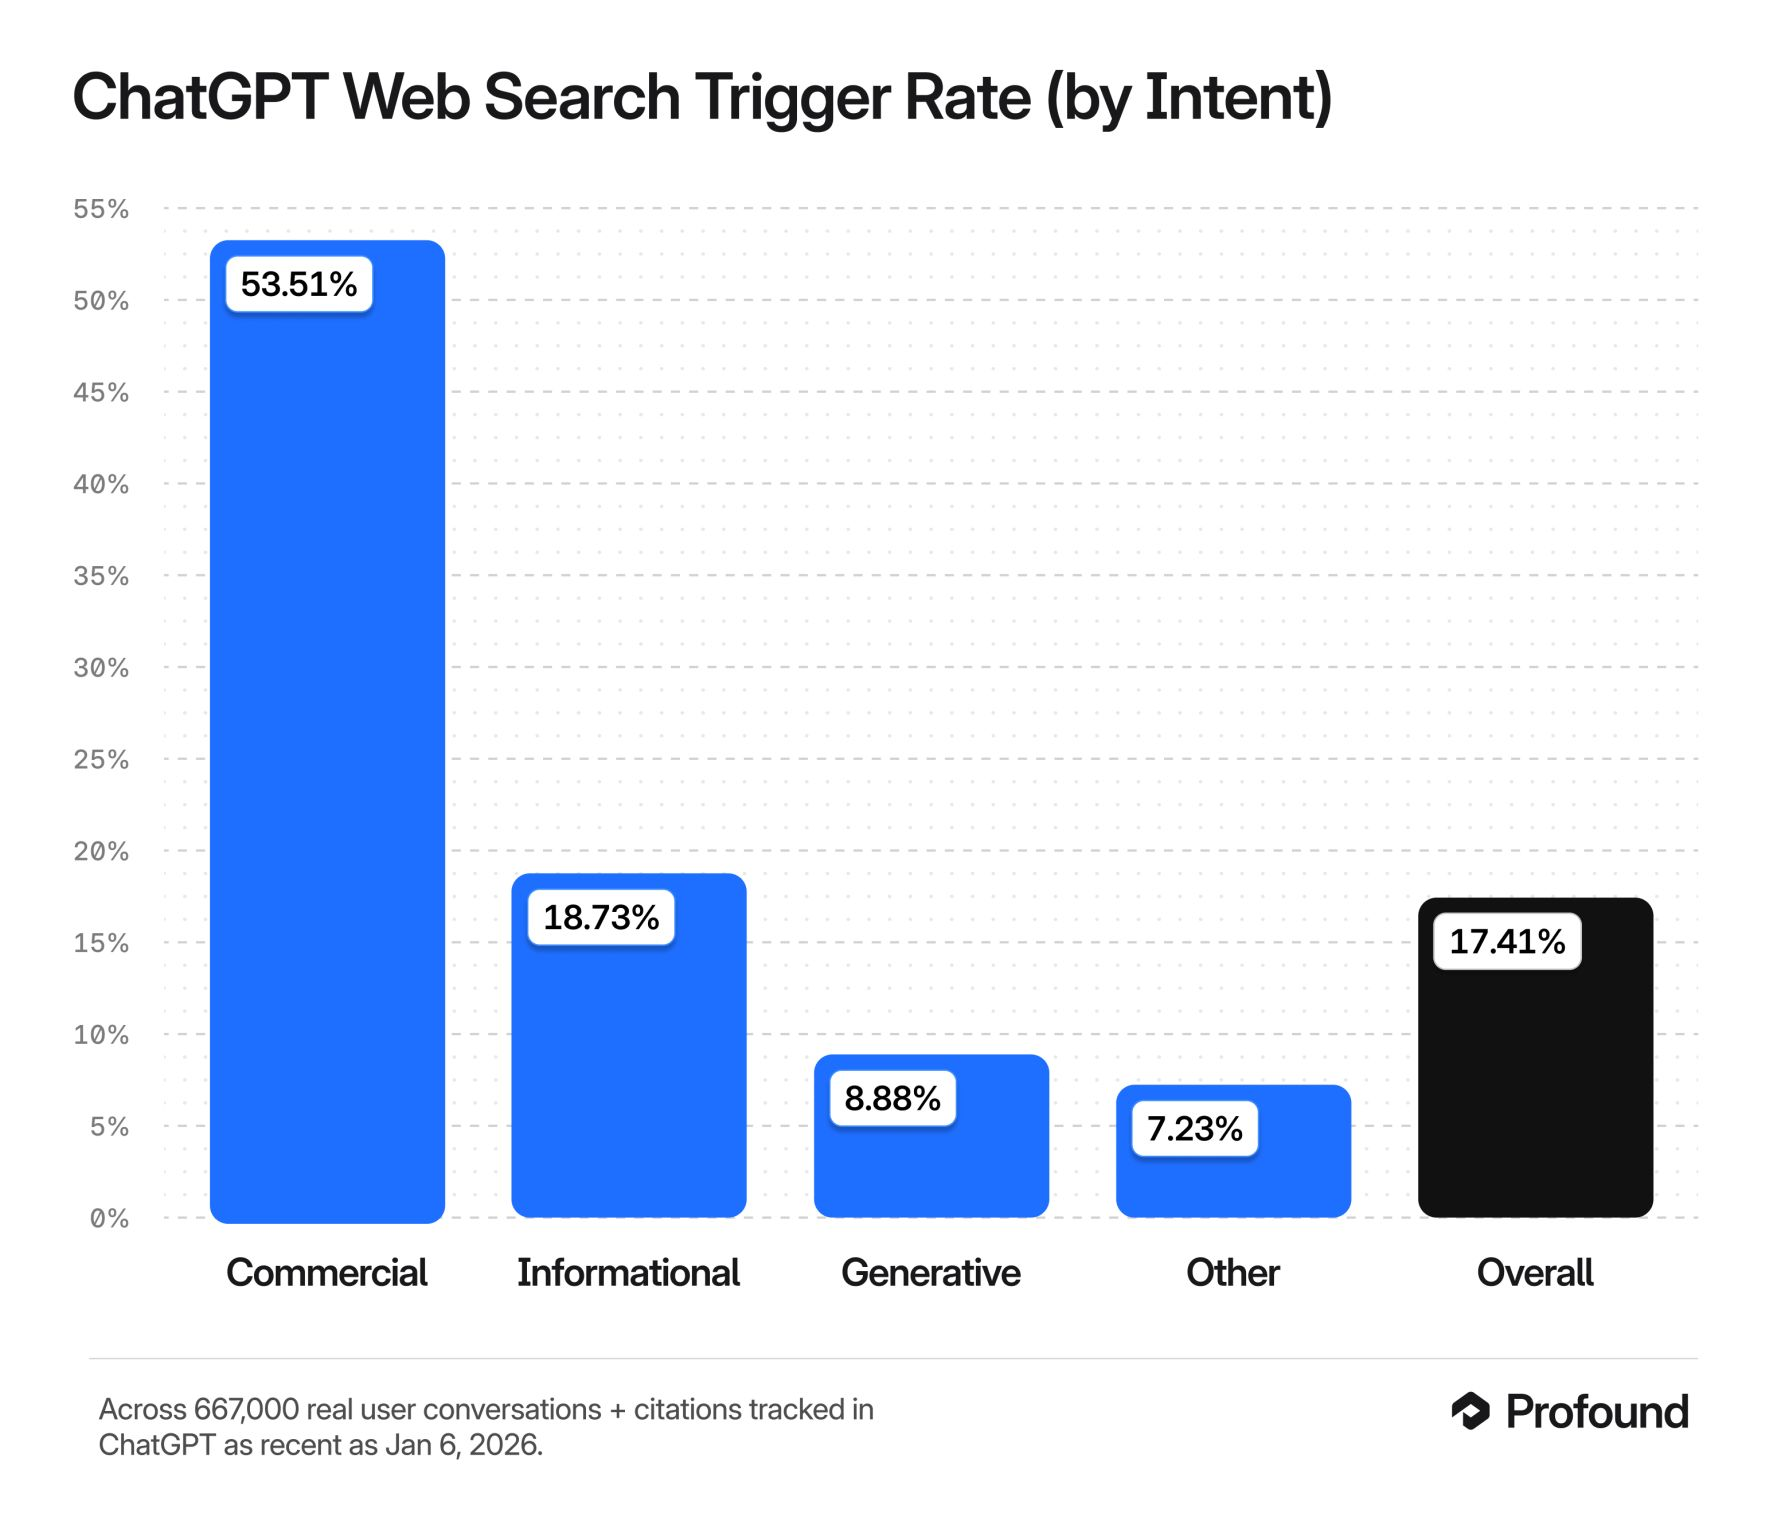
\includegraphics[width=\textwidth]{figures/1767882183827.jpg}
    \caption{ChatGPT Web Search Trigger Rate (by Intent)}
    \label{fig:trigger-rate}
\end{figure}

\begin{itemize}
    \item \textbf{Commercial Intent as the Primary Driver}: Web search is triggered in \textbf{53.51\% of Commercial queries}, compared to only 18.73\% for Informational and 8.88\% for Generative queries.
    \item \textbf{Overall Trigger Rate}: Across all intents, the baseline trigger rate is \textbf{17.41\%}.
    \item \textbf{Thesis Alignment}: Our decision to filter for \textbf{high commercial intent} (product recommendations) aligns with this industry data, as this is the segment where RAG/Grounding is most active and commercially impactful.
    \item \textbf{The ``Winnable'' Arena:} Because commercial intent requires real-time data (pricing, availability, reviews), it is the primary driver for RAG adoption. This makes product recommendations the most critical area for studying the shift from SEO to GEO.
\end{itemize}

\subsection{The GEO Industry Landscape: Citation Tracking \& ``Share of Model''}
\label{sec:geo-landscape}

\begin{itemize}
    \item \textbf{The Rise of GEO Analytics}: Emerging platforms (e.g., \textbf{Profound}, \textbf{Peec.ai}) are shifting the industry from ``Share of Voice'' (traditional search) to ``Share of Model'' (generative search).
    \item \textbf{The Listicle as the ``Critical Node''}: Our research places extreme emphasis on listicles because they are the primary ``on-ramp'' for product citations. In the GEO ecosystem, being cited in a top-tier listicle is no longer just about referral traffic; it is a prerequisite for being ``seen'' by the RAG orchestrator.
    \item \textbf{Quantifying the Value of a Citation}: By measuring the \textbf{Bias Multiplier} (how much more likely a cited product is to be selected vs.\ a random one) and \textbf{Host Exclusion} (the risk of being ignored if you are the host), we provide the first empirical framework for what these citation-tracking tools are actually measuring.
    \item \textbf{The ``Gold Rush'' of AEO/GEO:} The rapid rise of companies like \textbf{Profound} and \textbf{Perplexity AI} underscores the industry's recognition that the ``Answer Engine'' is the next multi-billion dollar shift in tech.
    \item \textbf{Venture Capital Validation:} A landmark moment occurred on August 12, 2025, when \textbf{Profound raised \$35 million in a Series B round led by Sequoia Capital}, bringing its total funding to \$58.5 million\footnote{\url{https://fortune.com/2025/08/12/ai-search-startup-profound-raises-35-million-series-b-sequoia/}}.
    \item \textbf{The ``Salesforce of AI Search'':} This funding round validated the concept of building a ``generational company'' centered on helping brands monitor and optimize for how they surface in AI-generated responses across models like ChatGPT, Gemini, and Claude.
    \item \textbf{The European Challenger --- Peec AI:} In November 2025, Berlin-based \textbf{Peec AI} raised \textbf{\$21 million in a Series A led by Singular}, bringing its total funding to \$29 million\footnote{\url{https://techcrunch.com/2025/11/17/as-consumers-ditch-google-for-chatgpt-peec-ai-raises-21m-to-help-brands-adapt/}}. Founded in early 2025, Peec grew to \textbf{\$4M ARR in 10 months} with 1,300 companies on its platform (including ElevenLabs, Chanel, and Axel Springer), explicitly positioning itself in the \textbf{Generative Engine Optimization (GEO)} category. The speed of Peec's traction---alongside Profound's Sequoia-backed round---confirms that AI search analytics is rapidly consolidating into a recognized market category, not a niche experiment.
    \item \textbf{The Hype vs.\ Reality:} While the hype is centered on ``killing search,'' our research suggests the reality is a \textbf{deeper integration} where search becomes the infrastructure for AI.
    \item \textbf{The High-Intent Conversion Hypothesis}: Preliminary industry observations suggest that while AI-driven traffic volume is currently lower than traditional search, the \textbf{conversion rate} and \textbf{purchase intent} of LLM-referred users can be significantly higher---implying that LLM citations act as a ``pre-qualified'' lead source, making the mechanics of selection (which we study here) commercially critical.
\end{itemize}

\section{Retrieval Environments \& Deployment Contexts}
\label{sec:retrieval-environments}

\textit{Defining the specific interfaces and constraints of the models under study.}

\subsection{ChatGPT: UI-Based Network Instrumentation (Personal vs.\ Enterprise)}
\label{sec:chatgpt-instrumentation}

\begin{itemize}
    \item \textbf{Deployment Context}: We study ChatGPT as a consumer-facing product accessed via the standard web interface (\texttt{chatgpt.com}).
    \item \textbf{Instrumentation Method}: Because OpenAI does not expose grounding metadata (fan-out queries, retrieved snippets) via its public API, we used \textbf{Network Payload Inspection} (Chrome DevTools protocol) to capture the raw event stream of the production UI.
    \item \textbf{Session Isolation}: All ChatGPT prompt runs were conducted in \textbf{Temporary Chat} mode to prevent conversation history and memory from influencing retrieval or generation behavior across runs.
    \item \textbf{Personal vs.\ Enterprise}:
    \begin{itemize}
        \item \textbf{Personal}: Executed on a \textbf{ChatGPT Plus} subscription in the user's \textbf{personal workspace}. OpenAI's general documentation\footnote{\url{https://openai.com/index/introducing-chatgpt-search/}} describes ChatGPT search as leveraging ``third-party search providers'' (plural), leaving the exact provider mix unspecified.
        \item \textbf{Enterprise}: Executed through a \textbf{ChatGPT Enterprise organization account}. OpenAI's Enterprise documentation\footnote{\url{https://help.openai.com/en/articles/10093903-chatgpt-search-for-enterprise-and-edu}} explicitly names \textbf{Bing} as the search provider, restricting retrieval to the Azure/Bing ecosystem.
    \end{itemize}
\end{itemize}

\subsection{Gemini: API-Based Grounding (Vertex AI)}
\label{sec:gemini-instrumentation}

\begin{itemize}
    \item \textbf{Deployment Context}: Unlike ChatGPT, Gemini was studied via the \textbf{Vertex AI / Google AI Studio API} (Gemini 1.5 Pro/Flash).
    \item \textbf{Instrumentation Method}: We utilized the API specifically to access the \textbf{\texttt{groundingMetadata}} object, which is not fully transparent in the consumer UI.
    \item \textbf{Reliability of Data}: The API provides a `cleaner' laboratory environment, exposing the exact \texttt{groundingChunks} (retrieved snippets) and \texttt{groundingSupports} (segment-to-chunk mapping) required for high-fidelity grounding analysis.
\end{itemize}
